\documentclass[12pt,a4paper]{article}

% ─── Page Layout ───────────────────────────────────────────────────────────────
\usepackage[a4paper, margin=0.8in, headheight=14pt]{geometry}

% ─── Fonts (XeLaTeX) ───────────────────────────────────────────────────────────
\usepackage{fontspec}
\usepackage{unicode-math}
\setmainfont{TeX Gyre Pagella}
\setmonofont[Scale=0.88]{TeX Gyre Cursor}
\setmathfont{Latin Modern Math}

% ─── Packages ──────────────────────────────────────────────────────────────────
\usepackage{xcolor}
\usepackage{colortbl}
\usepackage{titlesec}
\usepackage{enumitem}
\usepackage{tabularx}
\usepackage{booktabs}
\usepackage{array}
\usepackage{amsmath}
\usepackage{tikz}
\usetikzlibrary{shapes.geometric, arrows.meta, positioning, calc, fit}
\usepackage{tcolorbox}
\tcbuselibrary{skins, breakable}
\usepackage{hyperref}
\usepackage{fancyhdr}
\usepackage{graphicx}
\usepackage{microtype}
\hyphenpenalty=10000
\exhyphenpenalty=10000
\sloppy
\usepackage{caption}
\usepackage{setspace}
\usepackage{multirow}
\usepackage{tocloft}

% ─── Q&A helper ────────────────────────────────────────────────────────────────
\newcommand{\Q}[1]{\textbf{#1}\par\noindent\ignorespaces}

% ─── Colour Palette ────────────────────────────────────────────────────────────
\definecolor{myred}{RGB}{196,30,58}
\definecolor{mydark}{RGB}{30,30,50}
\definecolor{mygreen}{RGB}{14,120,80}
\definecolor{myteal}{RGB}{0,130,140}
\definecolor{myamber}{RGB}{180,100,0}
\definecolor{mypurple}{RGB}{100,30,160}
\definecolor{mygray}{RGB}{246,247,249}
\definecolor{mgframe}{RGB}{180,185,200}
\definecolor{watermark}{RGB}{145,150,170}
\definecolor{hdrred}{RGB}{250,232,235}
\definecolor{hdrgreen}{RGB}{220,244,233}
\definecolor{hdrteal}{RGB}{220,242,244}
\definecolor{hdramber}{RGB}{253,242,215}
\definecolor{hdrpurple}{RGB}{238,228,255}
\definecolor{hdrgray}{RGB}{238,240,245}
\definecolor{rowalt}{RGB}{250,251,253}

% ─── Section Formatting ────────────────────────────────────────────────────────
\titleformat{\section}
  {\large\bfseries\color{myred}}{\thesection.}{0.5em}{}
  [\vspace{1pt}{\color{myred}\rule{\linewidth}{0.8pt}}]
\titleformat{\subsection}
  {\normalsize\bfseries\color{myteal}}{\thesubsection}{0.5em}{}
\titlespacing*{\section}{0pt}{18pt}{7pt}
\titlespacing*{\subsection}{0pt}{11pt}{4pt}

\setlength{\parindent}{0pt}
\setlength{\parskip}{4pt}

% ─── TOC Styling ───────────────────────────────────────────────────────────────
\renewcommand{\cfttoctitlefont}{\large\bfseries\color{myred}}
\renewcommand{\cftaftertoctitle}{\par\noindent{\color{myred}\rule{\linewidth}{0.8pt}}}
\setlength{\cftbeforetoctitleskip}{0pt}
\setlength{\cftaftertoctitleskip}{6pt}
\renewcommand{\cftsecfont}{\normalsize\bfseries\color{mydark}}
\renewcommand{\cftsecpagefont}{\normalsize\bfseries\color{mydark}}
\renewcommand{\cftsecleader}{\cftdotfill{\cftdotsep}}
\setlength{\cftbeforesecskip}{7pt}
\renewcommand{\cftsubsecfont}{\small\color{mydark}}
\renewcommand{\cftsubsecpagefont}{\small\color{mydark}}
\setlength{\cftbeforesubsecskip}{3pt}
\setlength{\cftsubsecindent}{1.4em}

% ─── Table helpers ─────────────────────────────────────────────────────────────
\renewcommand{\arraystretch}{1.45}
\setlength{\tabcolsep}{6pt}
\arrayrulecolor{mydark}
\newcolumntype{B}[1]{>{\small\bfseries\raggedright\arraybackslash}m{#1}}
\newcolumntype{Y}{>{\small\raggedright\arraybackslash}X}
\renewcommand{\tabularxcolumn}[1]{m{#1}}

% ─── Header / Footer ───────────────────────────────────────────────────────────
\pagestyle{fancy}
\fancyhf{}
\fancyhead[L]{\small\color{myred}\textbf{EC602}\;\color{mydark}--- Computer Network}
\fancyhead[R]{\small\color{myteal}\textbf{Module 2 Notes}}
\fancyfoot[C]{\small\color{mydark}\thepage}
\fancyfoot[R]{\small\color{watermark}\textit{\copyright\ Biraj}}
\renewcommand{\headrulewidth}{0.5pt}
\renewcommand{\footrulewidth}{0.3pt}

% ─── Hyperref ──────────────────────────────────────────────────────────────────
\hypersetup{
  colorlinks=true, linkcolor=myteal, urlcolor=myteal,
  pdfauthor={Biraj Sarkar},
  pdftitle={EC602 --- Module 2 Notes}
}

% ─── tcolorbox styles ──────────────────────────────────────────────────────────
\tcbset{
  tikzbox/.style={colback=mygray, colframe=mgframe, boxrule=0.6pt, arc=4pt,
    left=8pt, right=8pt, top=6pt, bottom=6pt,
    colbacktitle=mgframe, coltitle=mydark, fonttitle=\small\bfseries},
  defbox/.style={colback=hdrgreen, colframe=mygreen, boxrule=0.8pt, arc=4pt,
    left=9pt, right=9pt, top=6pt, bottom=6pt,
    colbacktitle=mygreen, coltitle=white, fonttitle=\small\bfseries},
  formulabox/.style={colback=hdrteal, colframe=myteal, boxrule=0.8pt, arc=4pt,
    left=9pt, right=9pt, top=7pt, bottom=7pt,
    colbacktitle=myteal, coltitle=white, fonttitle=\small\bfseries},
  examplebox/.style={colback=hdramber, colframe=myamber, boxrule=0.8pt, arc=4pt,
    left=9pt, right=9pt, top=6pt, bottom=6pt,
    colbacktitle=myamber, coltitle=white, fonttitle=\small\bfseries},
  masonbox/.style={colback=hdrpurple, colframe=mypurple, boxrule=0.8pt, arc=4pt,
    left=9pt, right=9pt, top=6pt, bottom=6pt,
    colbacktitle=mypurple, coltitle=white, fonttitle=\small\bfseries},
  exambox/.style={colback=hdrpurple, colframe=mypurple, boxrule=1pt, arc=5pt,
    left=10pt, right=10pt, top=8pt, bottom=8pt,
    colbacktitle=mypurple, coltitle=white, fonttitle=\bfseries,
    breakable}
}
% Make all boxes breakable across pages
\tcbset{breakable}

% ─── TikZ styles ───────────────────────────────────────────────────────────────
\tikzset{
  block/.style={rectangle, draw=myteal, fill=hdrteal, text width=2.4cm, align=center,
    minimum height=0.95cm, font=\small, rounded corners=3pt, line width=0.7pt},
  netnode/.style={rectangle, draw=myteal, fill=hdrteal, text width=2.0cm, align=center,
    minimum height=0.8cm, font=\small, rounded corners=3pt, line width=0.7pt},
  arrow/.style={-Stealth, thick, color=mydark},
  redarrow/.style={-Stealth, thick, color=myred},
  line/.style={thick, color=mydark}
}

% ═══════════════════════════════════════════════════════════════════════════════
\begin{document}
% ═══════════════════════════════════════════════════════════════════════════════

\begin{center}
  {\LARGE\bfseries\color{myred} EC602 --- Computer Network}\\[5pt]
  {\normalsize\color{mydark} Semester VI \quad$\bullet$\quad 3L:0T:0P \quad$\bullet$\quad 3 Credits}\\[3pt]
  {\normalsize\color{myteal}\textbf{Module 2 Exam Notes}}\\[3pt]
  {\small\color{mydark} CGEC \;$|$\; B.Tech ECE (2023--27) \;$|$\; \textit{Biraj Sarkar}}
\end{center}
\vspace{2pt}
\noindent{\color{myred}\rule{\linewidth}{1.5pt}}
\vspace{2pt}
\hypersetup{linkcolor=mydark}
\tableofcontents
\hypersetup{linkcolor=myteal}
\newpage

%═══════════════════════════════════════════════════════════════════════════════
\section{Data Link Layer}
%═══════════════════════════════════════════════════════════════════════════════

\begin{tcolorbox}[defbox]
\textbf{Data Link Layer (Layer 2):} Responsible for \textit{node-to-node} delivery of frames. It handles framing, physical addressing (MAC), error detection/correction, and flow control between adjacent nodes.
\end{tcolorbox}

\subsection{Types of Errors}

\begin{tabularx}{\linewidth}{|B{3.0cm}|X|}
\hline
\multicolumn{1}{|>{\centering\arraybackslash}p{3.0cm}|}{\textbf{\color{mygreen}Error Type}} &
\multicolumn{1}{>{\centering\arraybackslash}X|}{\textbf{\color{mygreen}Description}} \\
\hline
Single-bit error   & Only one bit in the data unit is changed (0 to 1 or 1 to 0). Rare in serial transmission. \\
\hline
Burst error        & Two or more consecutive bits are corrupted. More common; caused by noise bursts. Length = from first to last corrupted bit. \\
\hline
\end{tabularx}

\subsection{Framing}

\begin{tcolorbox}[defbox]
\textbf{Framing:} The process of dividing a stream of bits from the network layer into manageable data units called \textbf{frames}. Allows the receiver to identify the start and end of each frame.
\end{tcolorbox}

\subsubsection*{Character (Byte) Stuffing}
Used when frames contain text data. A special \textbf{flag byte} (e.g.\ \texttt{FLAG}) marks frame boundaries. If the flag byte appears in the data, an \textbf{escape byte (ESC)} is inserted before it.
\begin{itemize}[leftmargin=*, itemsep=2pt]
  \item If data contains \texttt{FLAG}: insert \texttt{ESC} before it.
  \item If data contains \texttt{ESC}: insert another \texttt{ESC} before it.
  \item Receiver removes the stuffed \texttt{ESC} bytes.
\end{itemize}

\subsubsection*{Bit Stuffing}
Used in bit-oriented protocols (e.g.\ HDLC). Flag pattern is \texttt{01111110}. To prevent this pattern from appearing in data:
\begin{itemize}[leftmargin=*, itemsep=2pt]
  \item \textbf{Sender:} After every 5 consecutive 1s in data, insert a 0.
  \item \textbf{Receiver:} After every 5 consecutive 1s, if next bit is 0, remove it; if 1, it is a flag.
\end{itemize}

\subsection{Error Detection and Correction}

\subsubsection*{Parity Check}
\begin{tcolorbox}[formulabox, title={\textbf{Parity Check}}]
A single parity bit is appended to make the total number of 1s \textbf{even} (even parity) or \textbf{odd} (odd parity).\\
\textbf{Limitation:} Detects only \textit{odd} number of bit errors; cannot detect even-number errors or correct errors.
\end{tcolorbox}

\subsubsection*{Cyclic Redundancy Check (CRC)}
\begin{tcolorbox}[formulabox, title={\textbf{CRC --- Most Widely Used Error Detection}}]
\textbf{Concept:} Treat the data as a binary polynomial. Divide by a \textbf{generator polynomial} $G(x)$. Append the remainder (CRC bits) to the data.\\[4pt]
\textbf{Sender:}
\begin{enumerate}[label=\arabic*., leftmargin=*, itemsep=2pt, topsep=0pt]
  \item Append $r$ zeros to data ($r$ = degree of $G(x)$).
  \item Divide augmented data by $G(x)$ using modulo-2 division (XOR).
  \item Replace appended zeros with remainder $R(x)$ --- this is the CRC.
\end{enumerate}
\textbf{Receiver:} Divide received frame by $G(x)$. If remainder $= 0$, no error; else error detected.\\[4pt]
\textbf{Common generators:} CRC-8 ($x^8+x^2+x+1$), CRC-16, CRC-32 (Ethernet).
\end{tcolorbox}

\subsubsection*{Hamming Code (Error Correction)}
\begin{tcolorbox}[formulabox, title={\textbf{Hamming Code}}]
Adds \textbf{redundant parity bits} at positions that are powers of 2 ($p_1, p_2, p_4, p_8, \ldots$). Each parity bit covers specific data bits.\\[4pt]
\textbf{Minimum redundant bits:} For $m$ data bits, need $r$ parity bits such that $2^r \geq m + r + 1$.\\[4pt]
\textbf{Error correction:} Receiver recalculates parity bits; the binary value of failing parity positions gives the \textbf{error position} (syndrome). Flip that bit to correct.\\
\textbf{Capability:} Detects and corrects \textbf{single-bit errors}; detects (not corrects) double-bit errors.
\end{tcolorbox}

\subsection{Flow Control}

\begin{tcolorbox}[defbox]
\textbf{Flow Control:} Mechanism to prevent a fast sender from overwhelming a slow receiver. The receiver controls the rate at which the sender transmits data.
\end{tcolorbox}

\begin{tabularx}{\linewidth}{|B{3.0cm}|X|}
\hline
\multicolumn{1}{|>{\centering\arraybackslash}p{3.0cm}|}{\textbf{\color{myteal}Method}} &
\multicolumn{1}{>{\centering\arraybackslash}X|}{\textbf{\color{myteal}Description}} \\
\hline
Stop-and-Wait      & Sender sends one frame, waits for ACK before sending next. Simple but inefficient (low throughput). \\
\hline
Sliding Window     & Sender can transmit multiple frames (window size $W$) before needing ACK. Improves efficiency. \\
\hline
\end{tabularx}

\subsection{ARQ Protocols (Automatic Repeat reQuest)}

\begin{tcolorbox}[defbox]
\textbf{ARQ:} Error control mechanism combining error detection with retransmission. Uses ACK (acknowledgement) and NAK (negative acknowledgement) to ensure reliable delivery.
\end{tcolorbox}

\subsubsection*{Stop-and-Wait ARQ}
\begin{tcolorbox}[formulabox, title={\textbf{Stop-and-Wait ARQ}}]
Sender transmits one frame and starts a timer. Waits for ACK.\\
\textbf{If ACK received:} Send next frame.\\
\textbf{If NAK or timeout:} Retransmit the same frame.\\[4pt]
\textbf{Efficiency:} $\eta = \dfrac{1}{1 + 2a}$ where $a = \dfrac{T_p}{T_f}$ (propagation delay / frame transmission time).\\
\textbf{Drawback:} Very low efficiency for large $a$ (long links or short frames).
\end{tcolorbox}

\begin{tcolorbox}[tikzbox, title={Stop-and-Wait ARQ --- Message Flow}]
\centering
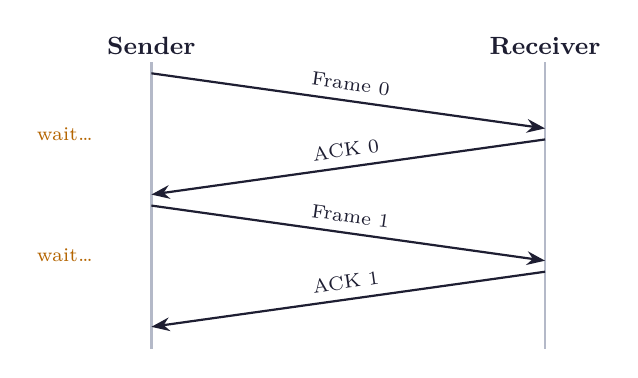
\begin{tikzpicture}[x=1cm, y=0.7cm,
  lbl/.style={font=\small\bfseries\color{mydark}}]
\node[lbl] at (0,5.5) {Sender};
\node[lbl] at (5,5.5) {Receiver};
\draw[thick,color=mgframe] (0,5.2) -- (0,0);
\draw[thick,color=mgframe] (5,5.2) -- (5,0);
% Frame 0
\draw[arrow] (0,5.0) -- node[above,sloped]{\scriptsize Frame 0} (5,4.0);
\draw[arrow] (5,3.8) -- node[above,sloped]{\scriptsize ACK 0} (0,2.8);
% Frame 1
\draw[arrow] (0,2.6) -- node[above,sloped]{\scriptsize Frame 1} (5,1.6);
\draw[arrow] (5,1.4) -- node[above,sloped]{\scriptsize ACK 1} (0,0.4);
% wait annotations
\node[font=\scriptsize\color{myamber}] at (-1.1,3.9) {wait\ldots};
\node[font=\scriptsize\color{myamber}] at (-1.1,1.7) {wait\ldots};
\end{tikzpicture}
\end{tcolorbox}

\subsubsection*{Go-Back-N ARQ (GBN)}
\begin{tcolorbox}[formulabox, title={\textbf{Go-Back-N ARQ}}]
Sender window size $W_s = 2^n - 1$ (for $n$-bit sequence numbers). Receiver window $W_r = 1$.\\
\textbf{On error:} Receiver discards the erroneous frame \textbf{and all subsequent frames}. Sender retransmits from the erroneous frame onwards.\\[4pt]
\textbf{Efficiency:} $\eta = \begin{cases} \dfrac{1}{1+2a} & \text{if } W \geq 1+2a \\ \dfrac{W}{1+2a} & \text{if } W < 1+2a \end{cases}$\\[4pt]
\textbf{Drawback:} Wastes bandwidth retransmitting correctly received frames.
\end{tcolorbox}

\subsubsection*{Selective Repeat ARQ (SR)}
\begin{tcolorbox}[formulabox, title={\textbf{Selective Repeat ARQ}}]
Sender window $W_s = 2^{n-1}$. Receiver window $W_r = 2^{n-1}$.\\
\textbf{On error:} Only the \textbf{erroneous frame} is retransmitted. Receiver buffers out-of-order frames.\\[4pt]
\textbf{Efficiency:} $\eta = \begin{cases} 1 & \text{if } W \geq 1+2a \\ \dfrac{W}{1+2a} & \text{if } W < 1+2a \end{cases}$\\[4pt]
\textbf{Advantage:} More efficient than GBN; \textbf{Disadvantage:} Requires larger receiver buffer.
\end{tcolorbox}

\begin{tabularx}{\linewidth}{|B{3.0cm}|X|X|X|}
\hline
\multicolumn{1}{|>{\centering\arraybackslash}p{3.0cm}|}{\textbf{Parameter}} &
\multicolumn{1}{>{\centering\arraybackslash}X|}{\textbf{Stop-and-Wait}} &
\multicolumn{1}{>{\centering\arraybackslash}X|}{\textbf{Go-Back-N}} &
\multicolumn{1}{>{\centering\arraybackslash}X|}{\textbf{Selective Repeat}} \\
\hline
Sender window   & 1             & $2^n - 1$     & $2^{n-1}$ \\
\hline
Receiver window & 1             & 1             & $2^{n-1}$ \\
\hline
On error        & Retransmit 1  & Retransmit from error & Retransmit only error \\
\hline
Efficiency      & Lowest        & Medium        & Highest \\
\hline
Buffer needed   & Minimal       & Small         & Large \\
\hline
\end{tabularx}

\subsection{HDLC (High-level Data Link Control)}

\begin{tcolorbox}[defbox]
\textbf{HDLC:} A bit-oriented, synchronous data link protocol developed by ISO. Uses bit stuffing for framing. Supports point-to-point and multipoint links.
\end{tcolorbox}

\textbf{HDLC Frame Structure:}\par\noindent
\begin{tabularx}{\linewidth}{|>{\centering\arraybackslash}X|>{\centering\arraybackslash}X|>{\centering\arraybackslash}X|>{\centering\arraybackslash}X|>{\centering\arraybackslash}X|}
\hline
\textbf{\color{myteal}Flag} & \textbf{\color{myteal}Address} & \textbf{\color{myteal}Control} & \textbf{\color{myteal}Data} & \textbf{\color{myteal}FCS + Flag} \\
\hline
01111110 & 8 bits & 8 or 16 bits & Variable & 16/32 bits + 01111110 \\
\hline
\end{tabularx}

\textbf{HDLC Frame Types:}
\begin{itemize}[leftmargin=*, itemsep=3pt]
  \item \textbf{I-frame (Information):} Carries user data; also piggybacks ACK.
  \item \textbf{S-frame (Supervisory):} Flow and error control (ACK, NAK, RNR).
  \item \textbf{U-frame (Unnumbered):} Link management (setup, disconnect).
\end{itemize}

%═══════════════════════════════════════════════════════════════════════════════
\section{Medium Access Sub-layer}
%═══════════════════════════════════════════════════════════════════════════════

\begin{tcolorbox}[defbox]
\textbf{Medium Access Control (MAC):} Sub-layer of the Data Link layer that controls how devices on a shared medium gain access to transmit. Prevents collisions and manages channel allocation.
\end{tcolorbox}

\subsection{Point-to-Point Protocol (PPP)}

\begin{tcolorbox}[defbox]
\textbf{PPP:} A byte-oriented protocol for direct serial links (e.g.\ dial-up, DSL). Provides framing, authentication, and network layer protocol negotiation.
\end{tcolorbox}

\textbf{PPP Components:}
\begin{itemize}[leftmargin=*, itemsep=3pt]
  \item \textbf{LCP (Link Control Protocol):} Establishes, configures, and tests the data link connection.
  \item \textbf{NCP (Network Control Protocol):} Configures network layer protocols (e.g.\ IPCP for IP). One NCP per network layer protocol.
\end{itemize}

\textbf{PPP Frame:} Flag (01111110) $|$ Address (FF) $|$ Control (03) $|$ Protocol $|$ Data $|$ FCS $|$ Flag

\subsection{Token Ring}

\begin{tcolorbox}[defbox]
\textbf{Token Ring (IEEE 802.4/802.5):} A deterministic MAC protocol where a special bit pattern called a \textbf{token} circulates around a ring. Only the station holding the token can transmit.
\end{tcolorbox}

\textbf{Operation:}
\begin{enumerate}[label=\textbf{\arabic*.}, leftmargin=*, itemsep=3pt]
  \item A free token circulates continuously around the ring.
  \item A station wishing to transmit captures the token, changes it to a \textit{busy token}, and appends its frame.
  \item The frame travels around the ring; the destination copies the data.
  \item The originating station removes the frame and releases a new free token.
\end{enumerate}
\textbf{Advantage:} Deterministic, no collisions, fair access. \textbf{Disadvantage:} Token loss/corruption disrupts network.

\begin{tcolorbox}[tikzbox, title={Token Ring Operation}]
\centering
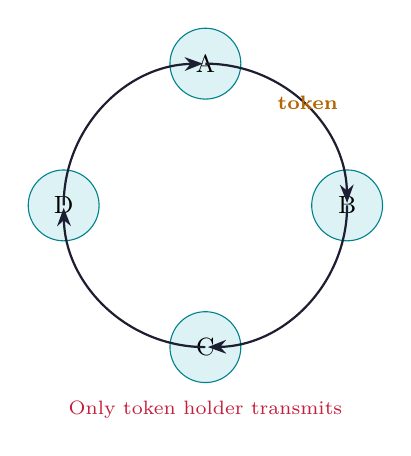
\begin{tikzpicture}[
  sta/.style={circle, draw=myteal, fill=hdrteal, minimum size=0.9cm, font=\small, align=center},
  tok/.style={font=\scriptsize\bfseries\color{myamber}}
]
\foreach \i/\lbl in {0/A, 1/B, 2/C, 3/D} {
  \pgfmathsetmacro\ang{90 - \i*90}
  \node[sta] (S\i) at (\ang:1.8cm) {\lbl};
}
\draw[arrow] (S0) arc[start angle=90, end angle=1, radius=1.8cm];
\draw[arrow] (S1) arc[start angle=0, end angle=-89, radius=1.8cm];
\draw[arrow] (S2) arc[start angle=270, end angle=181, radius=1.8cm];
\draw[arrow] (S3) arc[start angle=180, end angle=91, radius=1.8cm];
\node[tok] at (1.3,1.3) {token};
\node[font=\scriptsize\color{myred}, align=center] at (0,-2.6) {Only token holder transmits};
\end{tikzpicture}
\end{tcolorbox}

\subsection{Multiple Access Protocols}

\subsubsection*{Pure ALOHA}
\begin{tcolorbox}[formulabox, title={\textbf{Pure ALOHA}}]
Stations transmit whenever they have data. If collision occurs, wait a \textbf{random backoff time} and retransmit.\\[4pt]
\textbf{Throughput:} $S = G \cdot e^{-2G}$, maximum $S_{max} = \dfrac{1}{2e} \approx 18.4\%$ at $G = 0.5$.\\
\textbf{Vulnerable period:} $2T_f$ (two frame times).
\end{tcolorbox}

\subsubsection*{Slotted ALOHA}
\begin{tcolorbox}[formulabox, title={\textbf{Slotted ALOHA}}]
Time is divided into slots of size $T_f$. Stations can only transmit at the \textbf{beginning of a slot}.\\[4pt]
\textbf{Throughput:} $S = G \cdot e^{-G}$, maximum $S_{max} = \dfrac{1}{e} \approx 36.8\%$ at $G = 1$.\\
\textbf{Vulnerable period:} $T_f$ (one frame time) --- half that of Pure ALOHA.
\end{tcolorbox}

\subsubsection*{CSMA (Carrier Sense Multiple Access)}
\begin{tcolorbox}[defbox]
\textbf{CSMA:} Before transmitting, a station \textbf{senses the channel}. If busy, it waits; if idle, it transmits. Reduces (but does not eliminate) collisions due to propagation delay.
\end{tcolorbox}

\textbf{CSMA Variants:}\par\noindent
\begin{tabularx}{\linewidth}{|B{3.0cm}|X|}
\hline
\multicolumn{1}{|>{\centering\arraybackslash}p{3.0cm}|}{\textbf{\color{myteal}Variant}} &
\multicolumn{1}{>{\centering\arraybackslash}X|}{\textbf{\color{myteal}Behaviour on Busy Channel}} \\
\hline
1-persistent       & Wait until idle, then transmit immediately with probability 1. High collision risk. \\
\hline
Non-persistent     & Wait a random time, then sense again. Lower collision risk but higher delay. \\
\hline
p-persistent       & When idle, transmit with probability $p$, defer with probability $1-p$. Compromise. \\
\hline
\end{tabularx}

\subsubsection*{CSMA/CD (Collision Detection) --- Ethernet}
\begin{tcolorbox}[formulabox, title={\textbf{CSMA/CD}}]
Used in wired Ethernet (IEEE 802.3). Station senses channel; if idle, transmits and \textbf{monitors for collision simultaneously}.\\
\textbf{On collision:} Transmit jam signal, stop transmission, wait \textbf{binary exponential backoff} time, retry.\\[4pt]
\textbf{Backoff time:} $t = r \times T_{slot}$ where $r$ is random in $[0, 2^k - 1]$, $k$ = attempt number (max 10).\\
\textbf{Minimum frame size:} $L_{min} = 2 \times T_p \times B$ (to detect collision before frame ends).\\
\textbf{Not used in wireless} (cannot detect collision while transmitting).
\end{tcolorbox}

\begin{tcolorbox}[tikzbox, title={CSMA/CD Flowchart}]
\centering
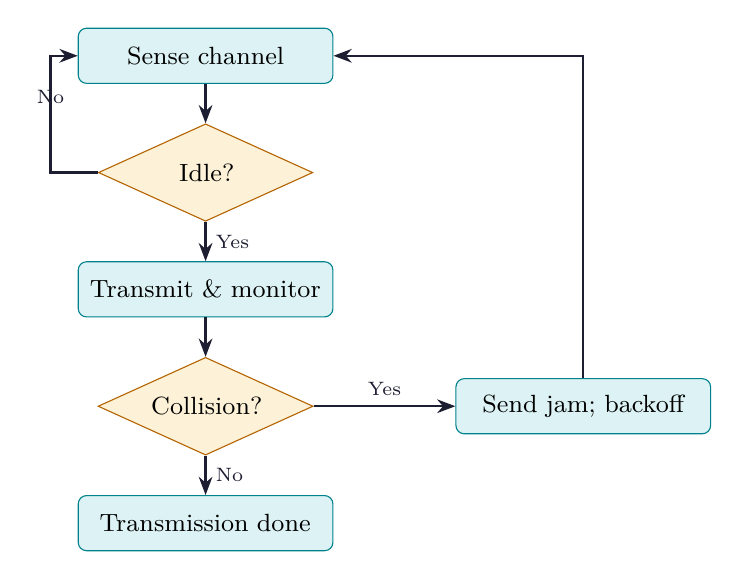
\begin{tikzpicture}[
  proc/.style={rectangle, draw=myteal, fill=hdrteal, text width=3.0cm, align=center, minimum height=0.7cm, font=\small, rounded corners=3pt},
  dec/.style={diamond, draw=myamber, fill=hdramber, text width=2.0cm, align=center, font=\small, aspect=2.2, inner sep=1pt},
  arr/.style={-Stealth, thick, color=mydark},
  node distance=0.5cm
]
\node[proc] (sense) {Sense channel};
\node[dec, below=0.5cm of sense] (idle) {Idle?};
\node[proc, below=0.5cm of idle] (tx) {Transmit \& monitor};
\node[dec, below=0.5cm of tx] (coll) {Collision?};
\node[proc, below=0.5cm of coll] (done) {Transmission done};
\node[proc, right=1.8cm of coll] (jam) {Send jam; backoff};

\draw[arr] (sense) -- (idle);
\draw[arr] (idle) -- node[right]{\scriptsize Yes} (tx);
\draw[arr] (idle.west) -- ++(-0.6,0) |- node[above,pos=0.25]{\scriptsize No} (sense.west);
\draw[arr] (tx) -- (coll);
\draw[arr] (coll) -- node[right]{\scriptsize No} (done);
\draw[arr] (coll) -- node[above]{\scriptsize Yes} (jam);
\draw[arr] (jam.north) |- (sense.east);
\end{tikzpicture}
\end{tcolorbox}

\subsubsection*{CSMA/CA (Collision Avoidance) --- Wi-Fi}
\begin{tcolorbox}[formulabox, title={\textbf{CSMA/CA}}]
Used in wireless networks (IEEE 802.11). Collision \textbf{avoidance} instead of detection (cannot detect collision in wireless).\\[4pt]
\textbf{Mechanism:}
\begin{enumerate}[label=\arabic*., leftmargin=*, itemsep=2pt, topsep=0pt]
  \item Sense channel; if idle for DIFS time, transmit.
  \item If busy, wait for channel to be idle, then wait a random \textbf{backoff} time.
  \item Transmit; receiver sends ACK after SIFS time.
  \item Optional: use \textbf{RTS/CTS} (Request to Send / Clear to Send) to reserve channel.
\end{enumerate}
\end{tcolorbox}

\subsection{Traditional and Fast Ethernet}

\begin{tabularx}{\linewidth}{|B{3.0cm}|X|X|}
\hline
\multicolumn{1}{|>{\centering\arraybackslash}p{3.0cm}|}{\textbf{Parameter}} &
\multicolumn{1}{>{\centering\arraybackslash}X|}{\textbf{\color{myteal}Traditional Ethernet (10 Mbps)}} &
\multicolumn{1}{>{\centering\arraybackslash}X|}{\textbf{\color{myamber}Fast Ethernet (100 Mbps)}} \\
\hline
Standard        & IEEE 802.3                    & IEEE 802.3u \\
\hline
Speed           & 10 Mbps                       & 100 Mbps \\
\hline
MAC protocol    & CSMA/CD                       & CSMA/CD \\
\hline
Frame format    & Same as 802.3                 & Same as 802.3 \\
\hline
Media           & Coaxial, UTP, fibre           & UTP Cat5, fibre \\
\hline
Variants        & 10Base2, 10Base5, 10BaseT     & 100BaseTX, 100BaseT4, 100BaseFX \\
\hline
\end{tabularx}

%═══════════════════════════════════════════════════════════════════════════════
% QUICK REVISION PAGE
%═══════════════════════════════════════════════════════════════════════════════
\newpage
\begin{center}
  {\large\bfseries\color{myred} Quick Revision --- Module 2}\\[3pt]
  {\small\color{mydark} Data Link Layer \& Medium Access Sub-layer $|$ EC602}
\end{center}
\noindent{\color{myred}\rule{\linewidth}{1.2pt}}
\vspace{4pt}

\begin{tcolorbox}[formulabox, title={\textbf{Key Formulas at a Glance}}]
\begin{tabularx}{\linewidth}{B{5.0cm} X}
Stop-and-Wait efficiency    & $\eta = \dfrac{1}{1+2a}$, \quad $a = T_p / T_f$ \\[4pt]
GBN efficiency              & $\eta = \dfrac{W}{1+2a}$ if $W < 1+2a$, else $1$ \\[4pt]
SR efficiency               & $\eta = \dfrac{W}{1+2a}$ if $W < 1+2a$, else $1$ \\[4pt]
GBN sender window           & $W_s = 2^n - 1$ \\[2pt]
SR sender/receiver window   & $W_s = W_r = 2^{n-1}$ \\[2pt]
Pure ALOHA max throughput   & $S_{max} = 1/(2e) \approx 18.4\%$ \\[2pt]
Slotted ALOHA max throughput& $S_{max} = 1/e \approx 36.8\%$ \\[2pt]
Hamming redundant bits      & $2^r \geq m + r + 1$ \\[2pt]
\end{tabularx}
\end{tcolorbox}

\vspace{6pt}

\begin{tcolorbox}[defbox, title={\textbf{One-Line Definitions}}]
\begin{itemize}[leftmargin=*, itemsep=3pt, topsep=0pt]
  \item \textbf{Framing:} Dividing bit stream into frames with identifiable start/end boundaries.
  \item \textbf{Bit Stuffing:} Inserting a 0 after five consecutive 1s to prevent flag pattern in data.
  \item \textbf{CRC:} Error detection using polynomial division; remainder appended as check bits.
  \item \textbf{Hamming Code:} Error-correcting code that adds parity bits at power-of-2 positions.
  \item \textbf{ARQ:} Automatic Repeat reQuest; error control using ACK/NAK and retransmission.
  \item \textbf{Go-Back-N:} On error, retransmit erroneous frame and all subsequent frames.
  \item \textbf{Selective Repeat:} On error, retransmit only the erroneous frame.
  \item \textbf{CSMA/CD:} Sense before transmit; detect collision and use backoff (Ethernet).
  \item \textbf{CSMA/CA:} Sense before transmit; avoid collision using backoff and ACK (Wi-Fi).
  \item \textbf{Token Ring:} Only the station holding the token can transmit; deterministic access.
  \item \textbf{PPP:} Point-to-Point Protocol; uses LCP for link setup and NCP for network config.
  \item \textbf{HDLC:} Bit-oriented DLL protocol; uses bit stuffing; I/S/U frame types.
\end{itemize}
\end{tcolorbox}

\vspace{6pt}

\begin{tcolorbox}[exambox, title={\textbf{Frequently Asked / Viva Questions}}]
\begin{enumerate}[leftmargin=*, topsep=0pt, label=\textbf{Q\arabic*.}, itemsep=8pt]
  \item \Q{What is the difference between burst error and single-bit error?} Single-bit: only one bit corrupted. Burst error: two or more consecutive bits corrupted; length measured from first to last corrupted bit.
  \item \Q{How does bit stuffing work in HDLC?} After every 5 consecutive 1s in data, sender inserts a 0. Receiver removes the stuffed 0 after 5 consecutive 1s.
  \item \Q{What is the maximum throughput of Pure ALOHA and Slotted ALOHA?} Pure ALOHA: $\approx 18.4\%$. Slotted ALOHA: $\approx 36.8\%$.
  \item \Q{Why is Slotted ALOHA more efficient than Pure ALOHA?} Vulnerable period is halved ($T_f$ vs.\ $2T_f$) because transmission is restricted to slot boundaries.
  \item \Q{What is the sender window size in Go-Back-N for 3-bit sequence numbers?} $W_s = 2^3 - 1 = 7$.
  \item \Q{Why can't CSMA/CD be used in wireless networks?} A wireless station cannot detect a collision while transmitting because its own signal overwhelms any incoming signal.
  \item \Q{What are LCP and NCP in PPP?} LCP establishes and configures the link. NCP configures the network layer protocol (e.g.\ IPCP for IP).
  \item \Q{What is the minimum frame size requirement in CSMA/CD?} Frame transmission time must be $\geq 2 \times$ propagation delay so the sender is still transmitting when the collision signal arrives.
  \item \Q{What are the three frame types in HDLC?} I-frame (data), S-frame (supervisory/flow control), U-frame (link management).
  \item \Q{What is binary exponential backoff?} After $k$-th collision, station waits a random time in $[0, 2^k - 1]$ slot times before retrying. Reduces repeated collisions.
  \item \Q{Difference between GBN and Selective Repeat?} GBN retransmits erroneous frame and all subsequent frames; SR retransmits only the erroneous frame. SR needs larger receiver buffer.
  \item \Q{What is the role of the MAC sub-layer?} Controls access to the shared transmission medium; prevents and manages collisions; provides physical addressing (MAC address).
\end{enumerate}
\end{tcolorbox}

\end{document}
